\chapter{Einleitung}
WAMS baut auf der Basis von \Gls{Apache Airflow} auf und erweitert bzw. ändert die Standardkonfiguration von Airflow ab, sodass der geforderte Funktionsumfang erreicht wird.
Dafür bringt WAMS ein eigenes Plugin mit, das weitere Webansichten und Operatoren einfügt.
Diese Ergänzungen ermöglichen es WAMS mehr Funktionalität über die Weboberfläche anzubieten.

Dass WAMS Airflow als Basis nutzt und darauf aufbaut, ergibt folgende Vorteile:
\begin{itemize}
    \item Die Funktionalität von Airflow bleibt erhalten, sodass WAMS ebenso mit dem Ökosystem von Airflow interagieren kann.
    \item Updates von Airflow können ohne Anpassung des WAMS-Plugins übernommen werden.
    \item Weite Teile der Deployment-Logistik Airflows werden übernommen.
\end{itemize}
Jedoch liefert Airflow noch nicht gesamten Funktionsumfang der von WAMS gefordert wird. Wie der geforderte Funktionsumfang erreicht wird, wird im Folgenden beschrieben.

%
%Dies ermöglicht das Apache Airflow unabhängig von WAMS aktualisiert werden kann.
%Dies verbessert die Erweiterbarkeit von WAMS durch die Installation von Airflow Plugins.
%Dies ermöglicht das WAMS erweiterbar ist durch die Installation von Airflow Plugins.
%Dies ermöglicht eine Verwendung von der aktuellen Airflow Version selbst bei updates.

\section{Paketstruktur}

%WAMS besteht aus zwei Hauptbestandteilen. In diesen sind Klassen mit ähnlichen Funktionen 
%zusammengefasst.
WAMS kann grob in zwei Bestandteile aufgeteilt werden:
\begin{itemize}
    \item Eine Airflow-Instanz mit spezieller Konfiguration
    \item Das eigene Plugin, welches die Weboberfläche von Airflow erweitert
\end{itemize}

Airflow bietet für Plugins eine eigene Schnittstelle an, die von WAMS genutzt wird, um eigene 
Webansichten hinzuzufügen. Da Airflow ab Version 2.0.0 für seine Weboberfläche und Nutzerverwaltung
das Flask AppBuilder Framework nutzt, werden die Ansichten von WAMS ebenso dieses Framework nutzen.

Für die Speicherung von Daten, die speziell von den Ansichten des WAMS-Plugin verwendet wird, bringt WAMS zusätzlich noch eine eigene Datenbank mit, die in einem eigenen Container läuft und über eine API von den Webansichten und Operatoren angesprochen wird.


Da WAMS eine Erweiterung von Airflow ist, werden unter anderem folgende Funktionen von Airflow übernommen:
\begin{itemize}
    \item Bestehende Weboberflächen
    \item Webserver
    \item Speicherung der Workflows
    \item Parametrierung der Workflows
    \item Datenbank für Metadaten
    \item Scheduling von Workflows
    \item Ausführung von Workflows
\end{itemize}
WAMS fügt zu Airflow Funktionen hinzu, die an verschiedene Komponenten Airflows anbinden und sie erweitern, wie in Grafik  \ref{fig:airflowÜbersicht} verdeutlicht wird. Aufgrund dieser Anknüpfung an verschiedenen Stellen, wird für das WAMS Plugin keine Model-View-Controller-Struktur verwendet.

\begin{figure}[H]
    \includegraphics[width=\textwidth]{Diagramme/Airflow übersicht.png}
    \caption{Anbindungsorte der Erweiterungen Airflows durch das WAMS Plugin. Farblich hervorgehoben sind die einzelnen Funktionspakete.\\ \tiny{Grundlegende Struktur Airflows übernommen von \nolinkurl{https://aws.amazon.com/de/blogs/machine-learning/build-end-to-end-machine-learning-workflows-with-amazon-sagemaker-and-apache-airflow/}}}
    \label{fig:airflowÜbersicht}
\end{figure}

%Da WAMS Airflow als Plugin erweitert und dieses an verschiedenen Stellen von Airflow anknüpft, wird für WAMS keine Model-View-Controller Struktur verwendet.
Zudem werden große Teile der Benutzeroberfläche von Airflow übernommen. 
Deswegen wird WAMS in Pakete aufgeteilt, welche jeweils einer Funktionalität von WAMS entsprechen. Diese Einteilung ermöglicht auch hohe Wiederverwendbarkeit der einzelnen Funktionen und verbessert so auch die Wartbarkeit.
%Da die Erweiterungen von WAMS an vielen Stellen des Modells von Airflow anbinden, wird für WAMS keine Model-View-Controller Struktur verwendet.

%Dabei liegt der Fokus auf einer Aufteilung in unterschiedliche Funktionen. 
%Das führt dazu, dass WAMS modular aufgebaut ist. 
%So können einzelne Funktionen von WAMS auch für andere ähnliche Plugins verwendet werden.
%Im Vergleich zur Aufteilung der Funktionen in mehrere Pakete ist dies durch die gewählte Paketstruktur einfach möglich.
%Es müssen lediglich die Pakete in ein anderes Plugin übernommen werden. 
Die Hauptaufgaben von WAMS liegen im Bereitstellen mehrere Funktionen in der Weboberfläche.
Folgende Pakete mit Funktionen stellt WAMS bereit:
\begin{itemize}
    \item Code Editor
    \item Result View
    \item Metadata Explorer
    \item Operators
    \item WAMSDatabase
\end{itemize}

\begin{figure}[h]
    \centering
    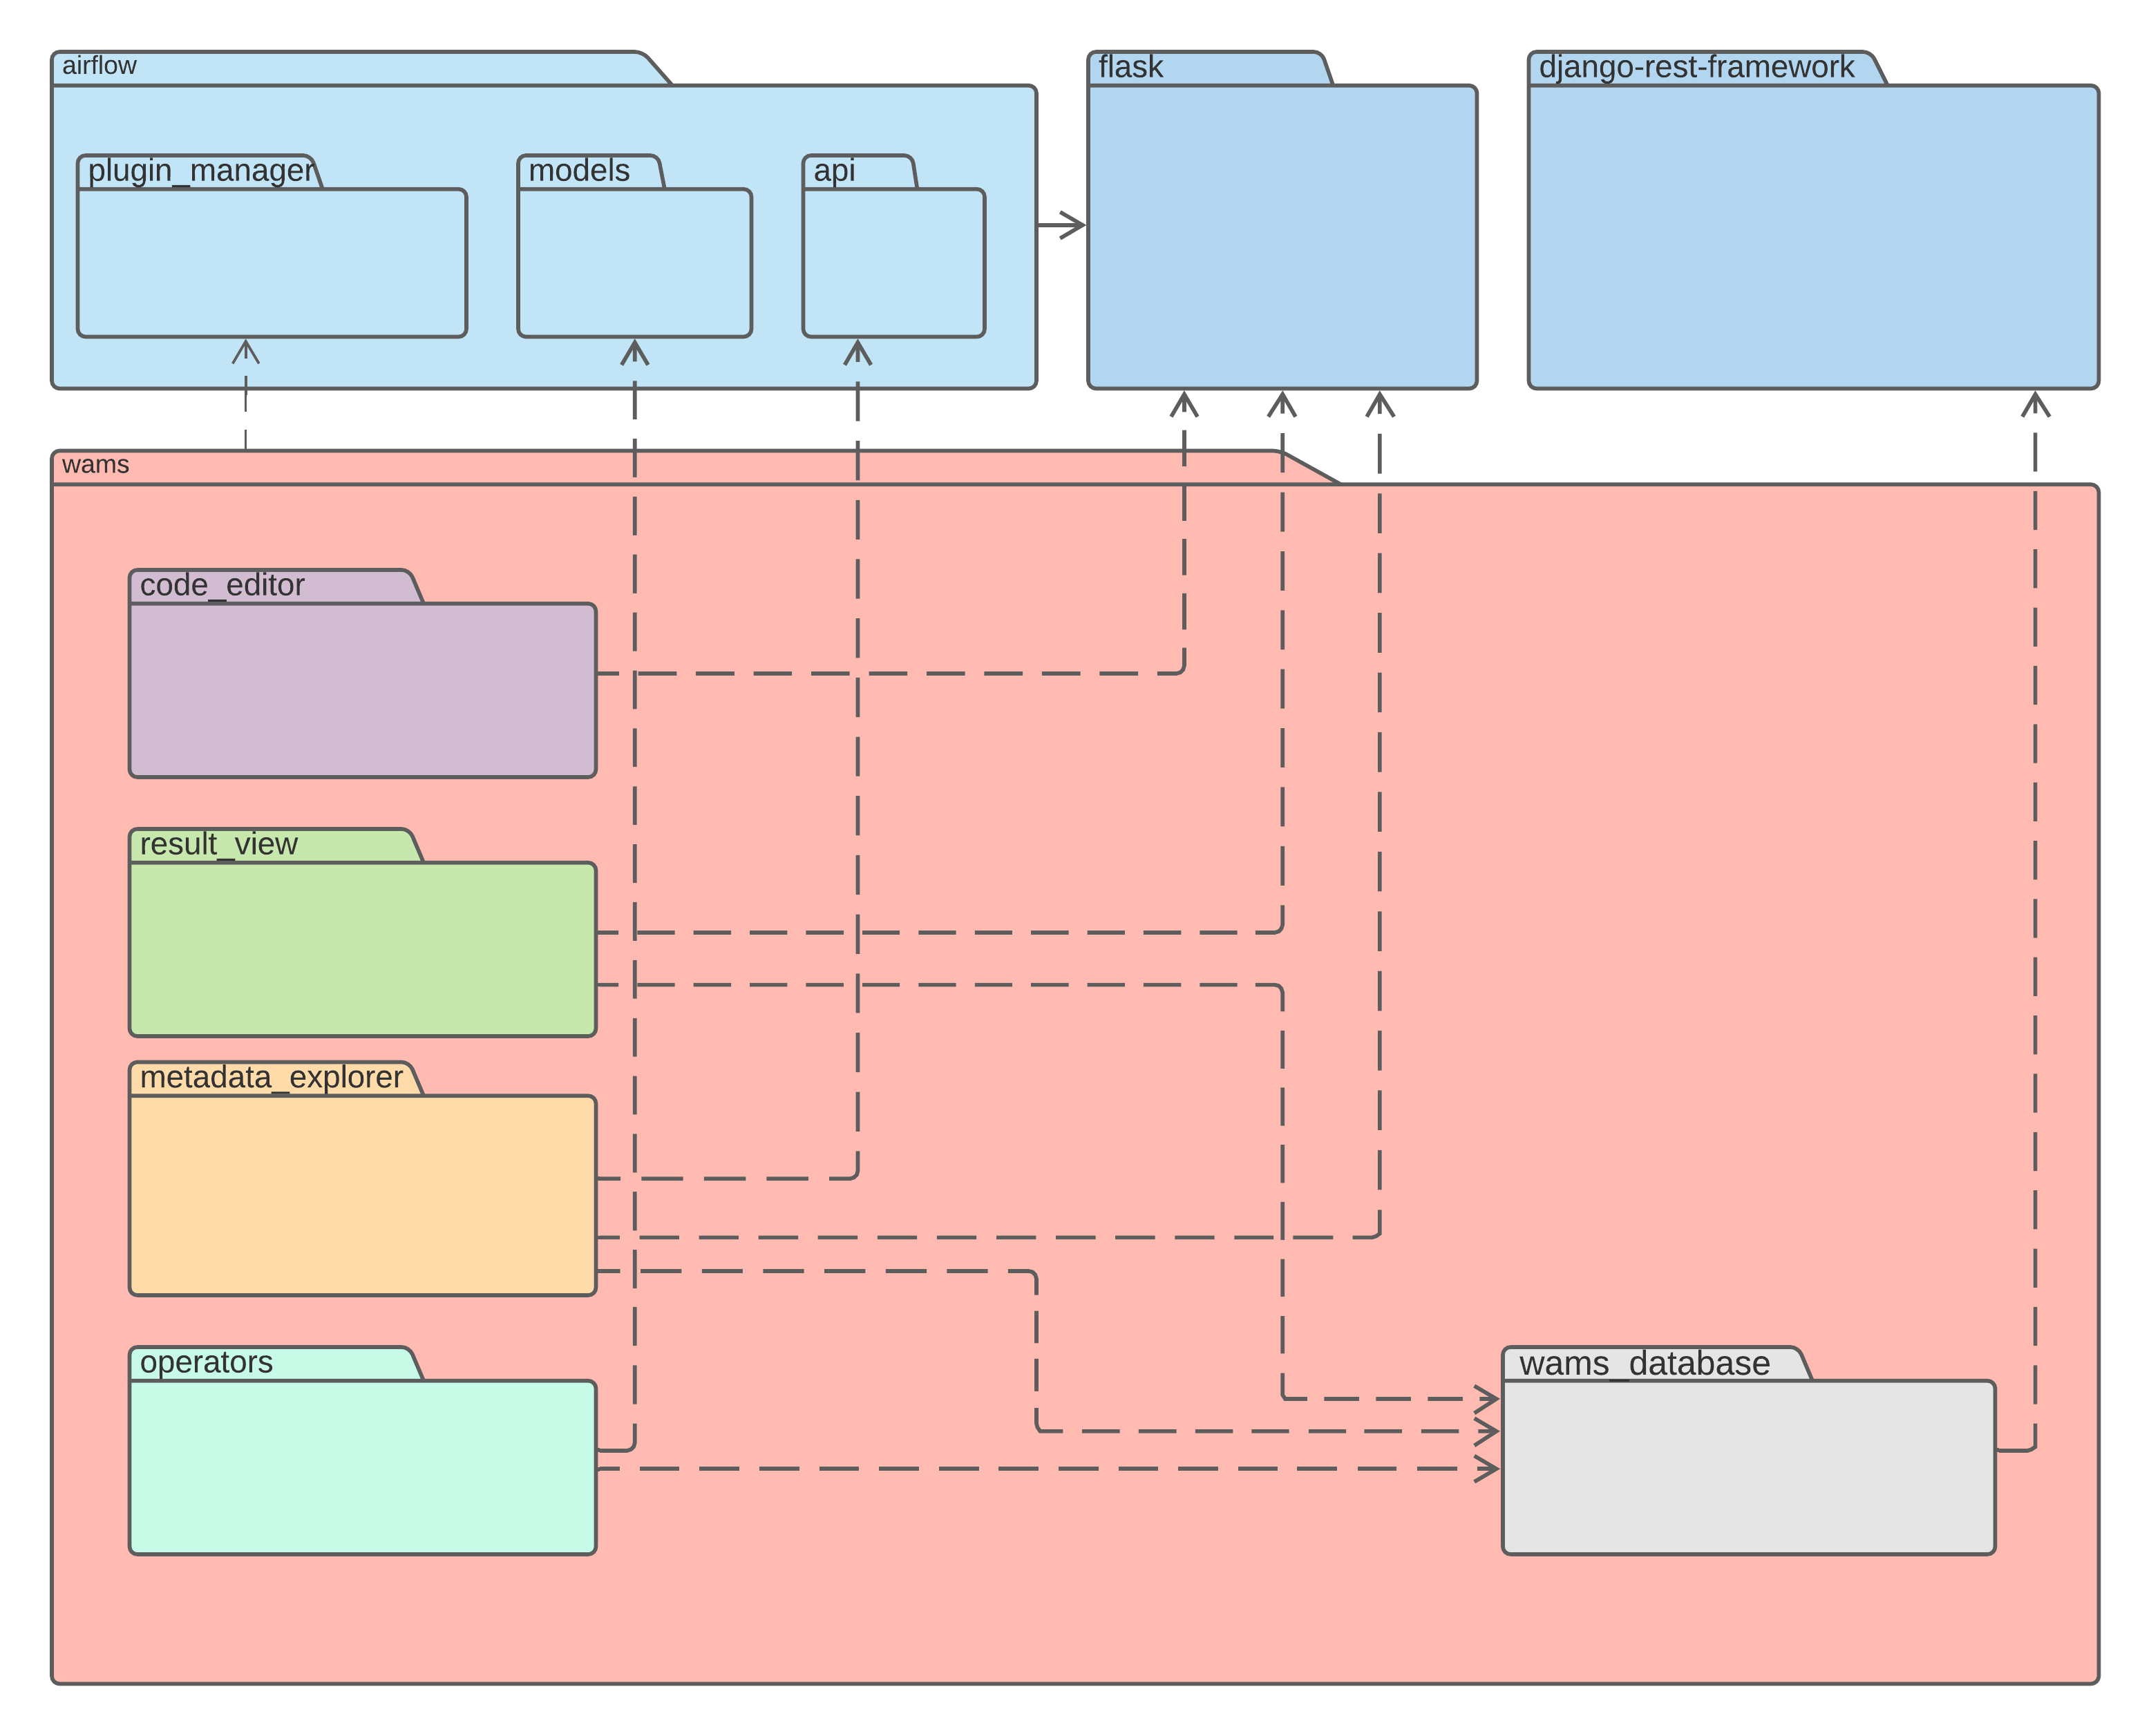
\includegraphics[width=\textwidth]{Diagramme/Paket.png}
    \caption{Paketdiagramm von WAMS}
    \label{fig:Paket}
\end{figure}

Diese Pakete werden in den nächsten Abschnitten einzeln behandelt.
Weiter greift WAMS auf mehrere Pakete innerhalb von Apache Airflow (\textit{airflow}) zu, insbesondere auf das Paket \textit{airflow.plugin\_manager} und auf das Paket \textit{airflow.api}. Das Paket \textit{airflow.plugin\_manager} liefert die Schnittstelle zur Einbindung des WAMS Plugins.
Das Paket \textit{airflow.api} enthält die Anwendungsprogrammierschnittstelle von Apache Airflow.

\subsection*{Code-Editor}
Der Code-Editor dient dazu den Python-Quellcode von Workflows in der Weboberfläche ändern zu können.
Hierbei wird das Airflow Plugin \gls{airflow-code-editor} von WAMS verwendet.

\subsection*{Result View}
Das Result View Paket erweitert die Weboberfläche von Airflow mit einem Tab zum Einsehen ausgewählter Ergebnisse und Zwischenergebnisse von Ausführungen von Workflows. 


\subsection*{Metadata Explorer}
Das Metadata Explorer Paket erweitert die Weboberfläche von Airflow durch einem Tab zum Einsehen der Metadaten einer Ausführung von Workflows. Die Metadaten werden über die Airflow API ermittelt.

\subsection*{Operators}
Das Operators Paket bündelt die in WAMS enthaltene Erweiterung der bereits in Apache Airflow existierenden Operatoren. 
In ihm sind Operatoren enthalten, die zu einer einfachen Anwendung von TGDS Workflows gedacht sind.
Außerdem ist ein Operator enthalten, der das Abspeichern von Ergebnissen und Zwischenergebnissen stark vereinfacht.

\subsection*{WAMSDatabase}
Das WAMSDatabase Paket ist zuständig für das Speichern von Daten im Zusammenhang mit Workflow-Instanzen.